%%%%%%%%%%%%%%%%%%%%%%%%%%%%%%%%%%%%%%%%%%%%%%%%%%%%%%%%%%%%%%%%%%%%%%%%%%%%%%%%%%%%%%%%%%%%%%%%
%
% CS576 Written Question Template
%
% Acknowledgements:
% The original code is written by Prof. James Tompkin (james_tompkin@brown.edu).
% The second version is revised by Prof. Min H. Kim (minhkim@kaist.ac.kr).
%
% This is a LaTeX document. LaTeX is a markup language for producing
% documents. Your task is to fill out this document, then to compile
% it into a PDF document.
%
%
% TO COMPILE:
% > pdflatex thisfile.tex
%
% If you do not have LaTeX and need a LaTeX distribution:
% - Personal laptops (all common OS): www.latex-project.org/get/
% - We recommend latex compiler miktex (https://miktex.org/) for windows,
%   macTex (http://www.tug.org/mactex/) for macOS users.
%   And TeXstudio(http://www.texstudio.org/) for latex editor.
%   You should install both compiler and editor for editing latex.
%   The another option is Overleaf (https://www.overleaf.com/) which is
%   an online latex editor.
%
% If you need help with LaTeX, please come to office hours.
% Or, there is plenty of help online:
% https://en.wikibooks.org/wiki/LaTeX
%
% Good luck!
% Min and the CS576 staff
%
%%%%%%%%%%%%%%%%%%%%%%%%%%%%%%%%%%%%%%%%%%%%%%%%%%%%%%%%%%%%%%%%%%%%%%%%%%%%%%%%%%%%%%%%%%%%%%%%
%
% How to include two graphics on the same line:
%
% \includegraphics[\width=0.49\linewidth]{yourgraphic1.png}
% \includegraphics[\width=0.49\linewidth]{yourgraphic2.png}
%
% How to include equations:
%
% \begin{equation}
% y = mx+c
% \end{equation}
%
%%%%%%%%%%%%%%%%%%%%%%%%%%%%%%%%%%%%%%%%%%%%%%%%%%%%%%%%%%%%%%%%%%%%%%%%%%%%%%%%%%%%%%%%%%%%%%%%

\documentclass[11pt]{article}

\usepackage[english]{babel}
\usepackage[utf8]{inputenc}
\usepackage[colorlinks = true,
            linkcolor = blue,
            urlcolor  = blue]{hyperref}
\usepackage[a4paper,margin=1.5in]{geometry}
\usepackage{stackengine,graphicx}
\usepackage{fancyhdr}
\setlength{\headheight}{15pt}
\usepackage{microtype}
\usepackage{times}
\usepackage{booktabs}

% From https://ctan.org/pkg/matlab-prettifier
\usepackage[numbered,framed]{matlab-prettifier}

\frenchspacing
\setlength{\parindent}{0cm} % Default is 15pt.
\setlength{\parskip}{0.3cm plus1mm minus1mm}

\pagestyle{fancy}
\fancyhf{}
\lhead{Homework Writeup}
\rhead{CS576}
\rfoot{\thepage}

\date{}

\title{\vspace{-1cm}Homework 5 Writeup}


\begin{document}
\maketitle
\vspace{-3cm}
\thispagestyle{fancy}

\section*{Instructions}
\begin{itemize}
  \item Describe any interesting decisions you made to write your algorithm.
  \item Show and discuss the results of your algorithm.
  \item Feel free to include code snippets, images, and equations.
  \item There is no page limit.

\end{itemize}

\section*{Feature extraction}
\begin{lstlisting}[language=Python]
import cv2
import numpy as np


def feature_extraction(img, feature):
    """
    This function computes defined feature (HoG, SIFT) descriptors of the target image.
	
    :param img: a height x width x channels matrix,
    :param feature: name of image feature representation.
	
    :return: a N x feature_size matrix.
    """
	
    if feature == 'HoG':
        # HoG parameters
        win_size = (32, 32)
        block_size = (32, 32)
        block_stride = (16, 16)
        cell_size = (16, 16)
        nbins = 9
        deriv_aperture = 1
        win_sigma = 4
        histogram_norm_type = 0
        l2_hys_threshold = 2.0000000000000001e-01
        gamma_correction = 0
        nlevels = 64
		
        # Your code here. You should also change the return value.
		
        hog_descriptor = cv2.HOGDescriptor(win_size, block_size, 
        block_stride, cell_size, nbins, deriv_aperture, win_sigma, 
        histogram_norm_type, l2_hys_threshold, gamma_correction, nlevels)
        feature = np.array(hog_descriptor.compute(img))
		
         return np.reshape(feature, ((int)(feature.shape[0]/36), 36))
	
    elif feature == 'SIFT':
	
        # Your code here. You should also change the return value.
		
        sift = cv2.SIFT_create()
        keypoints, descriptor = sift.detectAndCompute(img, None)
	
    return np.array(descriptor)
		
\end{lstlisting}

	I found features of images using hog and sift. 
	For HOG, Accuracy (mean of diagonal of confusion matrix) is 0.498
	For SIFT, Accuracy (mean of diagonal of confusion matrix) is 0.380
	SIFT should result better accuracy, so my implementation is not perfect. 

\section*{Principle component analysis (PCA) for vocabulary}
\begin{lstlisting}
import numpy as np

def get_features_from_pca(feat_num, feature):

    vocab = np.load(f'vocab_{feature}.npy')

    vocab_normalized = (vocab - vocab.mean(axis=0)) / vocab.std(axis=0)
    cov_vocab = vocab_normalized.T @ vocab_normalized
    _, eig_vec = np.linalg.eig(cov_vocab)

    return vocab_normalized @ (eig_vec[:, :feat_num] @ eig_vec[:, :feat_num].T)



\end{lstlisting}

I normalized the feature vectors of vocabularies, and performed PCA by finding eigen vectors. Image result below for HOG descriptor

\begin{figure}[h]
	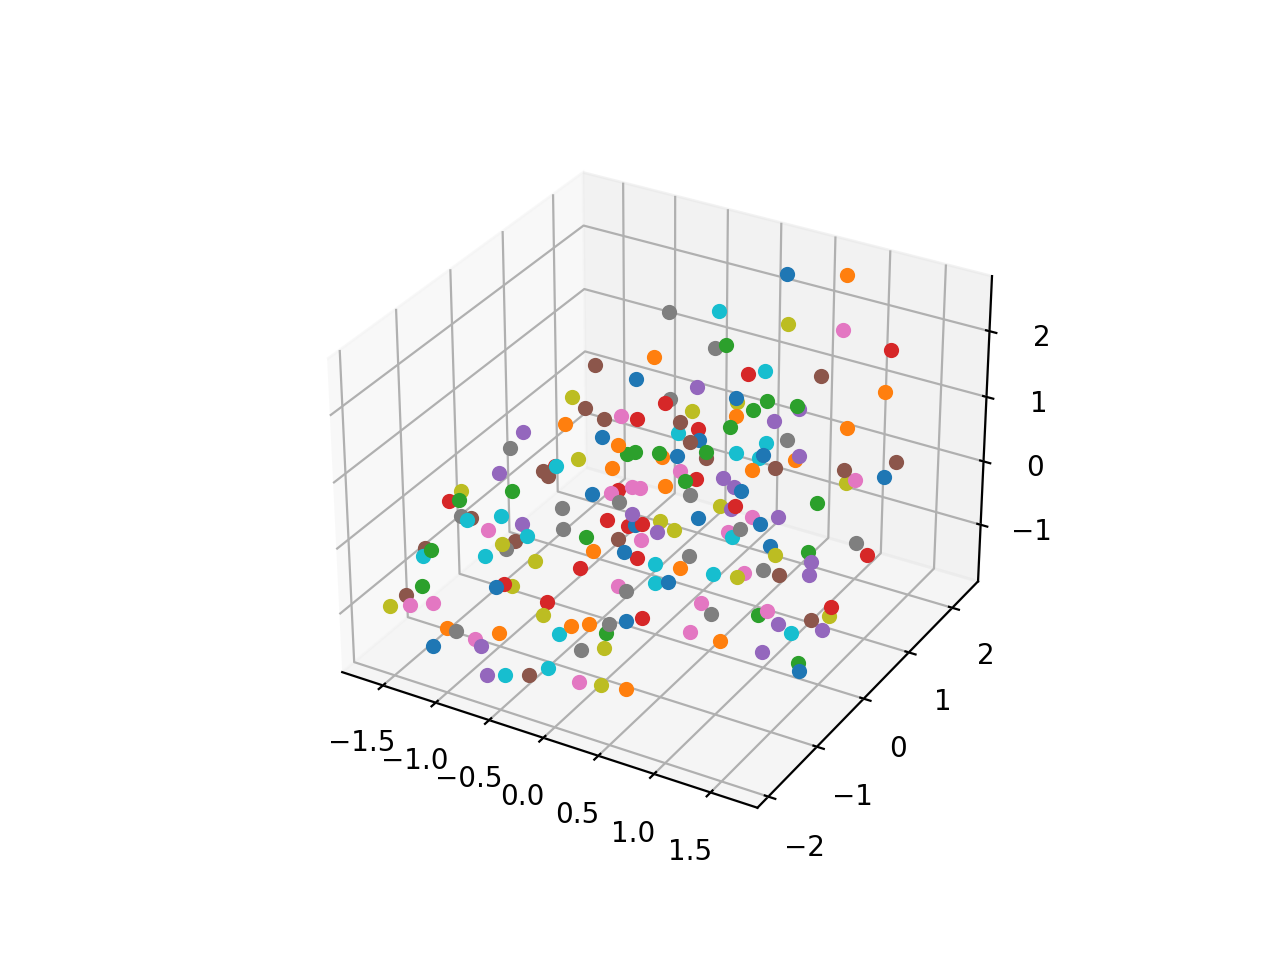
\includegraphics[width=5cm]{0.png}
\end{figure}

\section*{Bag of words representation of scenes}

\begin{lstlisting}
from matplotlib.pyplot import axis
import cv2
import numpy as np
from numpy import linalg

from distance import pdist
from feature_extraction import feature_extraction


def get_bags_of_words(image_paths, feature):
    vocab = np.load(f'vocab_{feature}.npy')

    vocab_size = vocab.shape[0]

    all_hists = []

    for path in image_paths:
        img = cv2.imread(path)[:, :, ::-1]

    features = feature_extraction(img, feature)
    hist, _ = np.histogram(np.argmin(pdist(features, vocab), axis=1), bins=[i for i in range(vocab.shape[0]+1)])
    hist = (hist - hist.mean()) / hist.std()
    all_hists.append(hist)

    return np.array(all_hists)
   
def get_spatial_pyramid_feats(image_paths, max_level, feature):

    vocab = np.load(f'vocab_{feature}.npy')

    vocab_size = vocab.shape[0]

    all_hists = []
    for path in image_paths:
        img = cv2.imread(path)[:, :, ::-1]
        img_hist = []
        w, h, _ = img.shape
        for i in range(max_level+1):
            for j in range(4**i):
                pyramid_img = img[w*(j//2**i)//2**i:w*(j//2**i+1)//2**i, h*(j%2**i)//2**i:h*(j%2**i+1)//2**i, :]
                features = feature_extraction(pyramid_img, feature)
                if features.shape == ():
                    hist = np.zeros(200)
                else:
                    hist, _ = np.histogram(np.argmin(pdist(features, vocab), axis=1), bins=[b for b in range(vocab.shape[0]+1)])
                    hist = (hist - hist.mean()) / hist.std()
        img_hist.append(hist) 
        img_hist = np.concatenate(img_hist, 0)
        all_hists.append(img_hist)

    return np.array(all_hists)
\end{lstlisting}
From the given words, find closest vocabulary and put it in the histogram. To find closest vocabulary, I computed distance between given word and vocabularies. 
For spatial pyramid representation, I splitted images for pyramid and extracted features from those image pieces, where bag of words compute it by extracting features of whole image. I used double loop to split image. 

Accuracy (mean of diagonal of confusion matrix) is 0.498 for HOG descriptor with bag of words method. 
Accuracy (mean of diagonal of confusion matrix) is 0.615 for HOG descriptor with spacial pyramid representation. 
Spacial pyramid representation should result in better accuracy, so my result corresponds with theory. 

\section*{SVM}
\begin{lstlisting}
from matplotlib.pyplot import axis
import numpy as np
from sklearn import svm


def svm_classify(train_image_feats, train_labels, test_image_feats, kernel_type):
    categories = np.unique(train_labels)

    score = []
    for label in categories:
        model = svm.LinearSVC(C=1, max_iter=100000)
        model.fit(train_image_feats, train_labels==label)
        score.append(model.decision_function(test_image_feats))
    score = np.array(score)
    classified_label = np.argmax(np.array(score), axis=0)

    return np.array([categories[i] for i in classified_label])
\end{lstlisting}

For all the labels, I computed SVM and its score to compare and get the best one, as shwon in "argmax"
For kernel trick, which I did not implemented, it projects data into higher-dimensional space defined by polynomials and Gaussian basis functions to fit for nonlinear relationships with a linear classifier. As a result, if implemented correctly, using RBF will increase accuracy. 


\end{document} 